% Provenance (never printed): see sources/outline_sources.md (Year 2: palaeogeography through
% the Phanerozoic; sea level; orogenies; mass extinctions and their Earth causes). Maps from the
% plate model of Merdith and others (2021) through the GPlates Web Service; sea level from the
% Miller and others (2005) NOAA study (Haq and others 1987; Kominz and others 2008); flooding and
% the Pitman model after Tasistro-Hart and Macdonald (2023); the big five after Marshall (2023)
% and Kaiho (2022); oceanic anoxic events after Rigo and others (2024) and Walker-Trivett and
% others (2024); CAMP carbon dioxide after Capriolo and others (2020); Chicxulub after
% Pickersgill and others (2026) and Collins and others (2020). Curves and numbers from
% figdata/bachelor-2/phanerozoic.py; exercise and problem values in the Book 4 scratch
% calculator calc/ch19.py.
\chapter{De fanerozoïsche Aarde}\label{ch:b2:phanerozoic-earth}

In het westen van Kansas, midden in Noord-Amerika, rijzen zuilen van wit krijt op uit de
prairie. Het krijt is het slib van een zeebodem: ongeveer 80 miljoen jaar geleden liep een
ondiepe zee van noord naar zuid door het midden van Noord-Amerika, en de schaaltjes van
zwevende algen bezonken op de bodem ervan met enkele honderdsten van een millimeter per jaar. Vijf keer in de
laatste 540 miljoen jaar verdween een groot deel van de soorten die in zulke zeeën leefden binnen een
geologisch ogenblik. Beide verhalen zijn die van de Aarde zelf: de continenten bewogen en de zee steeg en daalde over
hen heen, en minstens drie van de vijf grote uitstervingen vielen samen met uitvloeiingen van lava uit het binnenste van
de planeet. Dit hoofdstuk volgt het Fanerozoïcum aan de hand van zijn kaarten, zijn zeeniveau, zijn
gebergtegordels en zijn crises, en drukt er twee in getallen uit: hoe snel ruggen de zee doen stijgen, en hoeveel
land een hogere zee laat verdrinken.
% ledger: kgs:monument-rocks, kgs:chalk, ics:base.Phanerozoic, kaiho22:table, cr03:table

\begin{recall}
\textbf{Uit de schoolboeken}: platentektoniek en Pangea; fossielen en de geologische
tijdschaal; transgressies afgelezen in een klif. \textbf{Uit Boek~3}: de diepte--ouderdomswet van
de oceaanbodem; de hypsometrische curve; isostasie; eustasie en relatief zeeniveau; grote
stollingsprovincies; massa-uitstervingen als stratigrafische merkers, het iridium van de K--Pg-grens en de
datering van de crisis aan het einde van het Perm; etages en GSSP's. \textbf{Uit eerdere hoofdstukken}: \omterm{def:b2:alpine-orogen:orogen}{orogenen}
(\cref{ch:b2:alpine-orogen,ch:b2:himalaya-andes}); de \omterm{def:b2:wilson-cycle:wilson}{Wilsoncyclus} en \omterm{def:b2:wilson-cycle:supercontinent}{supercontinenten}
(\cref{ch:b2:wilson-cycle}); \omterm{def:b2:basins-compared:backstripping}{backstripping} (\cref{ch:b2:basins-compared}); de sneeuwballen van het
Cryogenium (\cref{ch:b2:precambrian-earth}). Uitsterven en de geschiedenis van het leven horen bij de
biologieboeken; Boek~5 behandelt paleomagnetisme en sequentiestratigrafie.
\end{recall}

\section{Kaarten van een bewegende wereld}\label{sec:b2:phanerozoic-earth:maps}

Een gesteente ligt zelden waar het ontstond. Een steenkool, een woestijnzandsteen, een rif: elk werd afgezet op
een bepaalde breedte en is sindsdien door zijn plaat meegevoerd. Voordat het klimaat of het leven van een vervlogen
tijd uit zulke gesteenten kan worden afgelezen, moeten ze worden teruggezet waar ze lagen.

\begin{definition}[Paleogeografie; paleogeografische kaart]\label{def:b2:phanerozoic-earth:palaeogeography}
\emph{Paleogeografie}\index{paleogeografie} is de reconstructie van de geografie van een vervlogen
tijd: de posities van de continenten en oceanen, en van hun kustlijnen, gebergtegordels en
zeeën. Een \emph{paleogeografische kaart}\index{paleogeografische kaart} toont die geografie op één
tijdstip, op het raster van breedte en lengte van dat tijdstip.
\end{definition}

Vier soorten bewijs gaan in zo'n kaart. De magnetisatie van gesteenten geeft de breedte waarop
ze ontstonden, het onderwerp van het paleomagnetisme in Boek~5; maar het veld van de Aarde is
symmetrisch rond haar as, dus het zegt niets over de lengte. De oceaanbodem legt de beweging van
de platen rechtstreeks vast, via zijn magnetische strepen en zijn ouderdommen, maar alleen tot aan de
oudste overgebleven bodem, ongeveer 190 miljoen jaar: alles wat ouder is, is gesubduceerd. Daarvoor
maken de passing van de continenten, de suturen en \omterm{def:b2:alpine-orogen:orogen}{orogenen} waar oceanen sloten, en de fossielen en
sedimenten die een klimaat verraden --- riffen en evaporieten in de tropen, glaciale afzettingen dicht bij de
polen --- het beeld compleet. Plaatmodellen verzamelen deze randvoorwaarden en draaien elke plaat terug in de
tijd; reconstructies moeten ook rekening houden met de trage rotatie van de hele vaste Aarde ten opzichte
van haar draaiingsas, de ware poolverschuiving.
% ledger: vh26:palaeogeography, gws:merdith-frame, data:b2-seafloor-age, merdith21:model

\begin{omfigure}
\centering
% figdata/bachelor-2/phanerozoic.py parts map-<t>, cities-<t>, grat (Mollweide, x and y in Earth radii)
\begin{tikzpicture}
\begin{groupplot}[group style={group size=2 by 3, horizontal sep=0.35cm, vertical sep=0.55cm},
  width=0.53\linewidth, axis equal image, hide axis, clip=false,
  xmin=-2.85, xmax=2.85, ymin=-1.43, ymax=1.43,
  title style={font=\small, yshift=-1.5ex}]
\pgfplotsinvokeforeach{500,300,200,100,50,0}{
\nextgroupplot[title={#1~\unit{Ma}}]
\fill[omSea] (axis cs:0,0) ellipse [x radius=2.8284, y radius=1.4142];
\addplot[fill=omLithAlluv!85!black, draw=none] table[x=x, y=y]
  {figdata/out/bachelor-2-phanerozoic-map-#1.dat};
\addplot[black!35, line width=0.2pt] table[x=x, y=y] {figdata/out/bachelor-2-phanerozoic-grat.dat};
\draw[black!70, line width=0.4pt] (axis cs:0,0) ellipse [x radius=2.8284, y radius=1.4142];
\addplot[only marks, mark=*, mark size=1.3pt, red!75!black, point meta=explicit symbolic,
  nodes near coords, nodes near coords style={font=\tiny\bfseries, anchor=south west,
  inner sep=0.5pt, text=red!60!black}]
  table[x=x, y=y, meta=tag] {figdata/out/bachelor-2-phanerozoic-cities-#1.dat};
}
\end{groupplot}
\end{tikzpicture}
\par\smallskip{\small De huidige kustlijnen teruggevoerd naar zes tijdstippen in het plaatmodel van
Merdith en anderen (2021), gereconstrueerd door de GPlates Web Service, in een oppervlaktegetrouwe
projectie van Mollweide; parallellen om de \ang{30}, meridianen om de \ang{60}. De rode stippen volgen vier
steden: Parijs (P), New York (N), Sydney (S) en Kaapstad (C, van Cape Town); op \qty{500}{Ma} zit de korst van
Sydney nog niet in het model. De vormen zijn de huidige kustlijnen, verplaatst, niet de kustlijnen van
die tijden, en in dit paleomagnetische referentiekader zijn de lengten willekeurig.}
\end{omfigure}
% ledger: data:b4-palaeocoast, data:b4-palaeopos, geonames4:cities, gws:merdith-frame, merdith21:model

De zes kaarten hierboven zijn het Fanerozoïcum in het kort. Op \qty{500}{Ma} vormen de zuidelijke continenten
één massa, Gondwana, waarvan een groot deel dicht bij de Zuidpool ligt, met de korst van Parijs op \ang{61}~ZB aan de
rand ervan. Tegen \qty{300}{Ma} zijn de continenten samengevoegd tot Pangea, gevormd vanaf ongeveer
\qty{325}{Ma} en uiteengebroken vanaf ongeveer \qty{200}{Ma}: Parijs en New York liggen op de evenaar, Kaapstad
en Sydney dicht bij \ang{60}~ZB. Op \qty{200}{Ma} is het \omterm{def:b2:wilson-cycle:supercontinent}{supercontinent} compleet, één enkel land
dat zich uitstrekt van hoge noordelijke tot hoge zuidelijke breedten; tegen \qty{100}{Ma} zijn de Atlantische en de Indische Oceaan opengegaan, en tegen
\qty{50}{Ma} is de kaart bijna de huidige, met Australië nog dicht bij Antarctica.
% ledger: data:b4-palaeopos, nance22:supercontinents

\begin{example}[Parijs drijft naar het noorden]\label{ex:b2:phanerozoic-earth:paris}
In het model lag Parijs \qty{300}{Ma} geleden op \ang{5.1}~NB; vandaag ligt het op \ang{48.9}~NB. Zijn
breedte is met \ang{43.8} gegroeid, dat wil zeggen $43.8 \times 111.2 = \qty{4871}{km}$ langs een meridiaan
($\qty{111.2}{km}$ per graad op een bol met straal \qty{6371}{km}), met een gemiddelde snelheid van
$4871/300 = \qty{16}{km}$ per miljoen jaar, of \qty{1.6}{cm} per jaar. Dit is alleen het noordwaartse
deel van de beweging: het paleomagnetische referentiekader laat de lengte vrij, dus de werkelijk afgelegde
afstand was minstens zo groot.
\end{example}
% ledger: data:b4-palaeopos, geonames4:cities, earth:Rmean, gws:merdith-frame
% values: calc/ch19.py (43.8 deg, 4870.6 km, 16.2 km/Myr)

\section{Het zeeniveau in de loop van het Fanerozoïcum}\label{sec:b2:phanerozoic-earth:sealevel}

\subsection*{Zeeën op de continenten}

Gedurende het grootste deel van het Fanerozoïcum lag veel meer van de continenten onder de zee dan vandaag. De
mariene gesteenten van Noord-Amerika leggen verscheidene overstromingen van het binnenland van het continent vast, de eerste
daarvan de cambrische transgressie die de Grote Discordantie afsluit; in het Laat-Krijt, van
ongeveer 120 tot \qty{80}{Ma}, hoopten zich mariene sedimenten op over het hele Western Interior, midden
in het continent (foto hieronder).
% ledger: th23:flooding, th23:wib

\begin{omfigure}
\centering
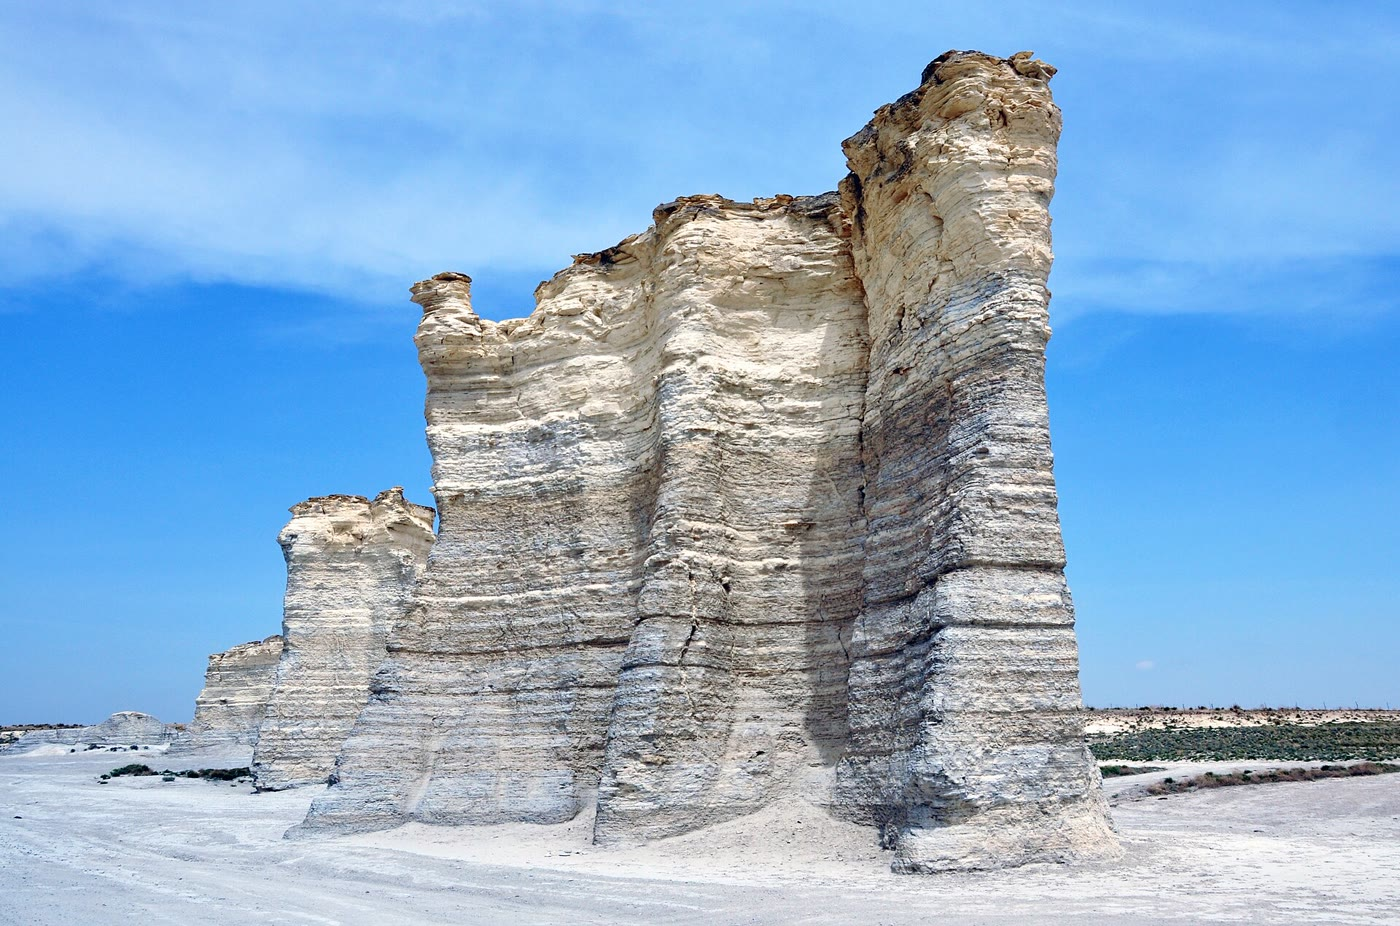
\includegraphics[width=0.66\linewidth]{images/book4/b2-19-monument-rocks.jpg}
\par\smallskip{\small Monument Rocks, westelijk Kansas: zuilen van krijt, het slib van een
krijtbinnenzee van ongeveer 80 miljoen jaar oud, afgezet met ongeveer \qty{0.036}{mm} per jaar. (James
St.~John, CC~BY~2.0, via Wikimedia Commons.)}
\end{omfigure}
% ledger: kgs:monument-rocks, kgs:chalk

\begin{definition}[Epicontinentale zee]\label{def:b2:phanerozoic-earth:epeiric}
Een \emph{epicontinentale zee}\index{epicontinentale zee} is een ondiepe zee die zich over het binnenland van een
continent uitspreidt, op continentale korst, ver van de continentale rand.
\end{definition}

De zee bereikt zulke binnenlanden door haar kust te verplaatsen, en de gesteenten leggen die beweging vast.

\begin{definition}[Mariene transgressie; mariene regressie]\label{def:b2:phanerozoic-earth:transgression}
Een \emph{mariene transgressie}\index{mariene transgressie} is een landwaartse verschuiving van de kustlijn,
waardoor de zee zich over het land uitspreidt; een \emph{mariene regressie}\index{mariene regressie} is
een zeewaartse verschuiving, waardoor het land opduikt.
\end{definition}

In een verticale doorsnede stapelt een transgressie afzettingen van dieper water op ondiepere ---
offshore-modder op strandzand --- en een regressie het omgekeerde. Beide volgen het relatieve
zeeniveau, dat het wereldwijde zeeniveau combineert met de daling of opheffing van de plaats en met de
aanvoer van sediment: een delta kan zijn kust zeewaarts duwen terwijl de zee stijgt, als hij snel genoeg
wordt gevoed. Om het wereldwijde zeeniveau uit transgressies af te lezen, moet een geoloog hetzelfde signaal
op verscheidene continenten vinden, of de daling verwijderen door \omterm{def:b2:basins-compared:backstripping}{backstripping}, zoals in
\cref{ch:b2:basins-compared}.
% ledger: miller20:rsl

\subsection*{De langetermijncurve}

\begin{definition}[Zeeniveaucyclus van de eerste orde]\label{def:b2:phanerozoic-earth:first-order}
De \emph{zeeniveaucyclus van de eerste orde}\index{zeeniveaucyclus van de eerste orde} is het traagste deel van
de verandering van het wereldwijde zeeniveau, op tijdschalen van tientallen tot honderden miljoenen jaren, bepaald door
de tektoniek van de vaste Aarde en niet door ijs.
\end{definition}

Over het Fanerozoïcum heeft de curve van de eerste orde de vorm van een M: hoog in het vroege Paleozoïcum,
laag terwijl Pangea zich vormde en bestond, van het Carboon tot het einde van het Trias, opnieuw hoog
in het Krijt, en dalend sindsdien. Geëxtrapoleerd vanuit Noord-Amerika wijst de overstroming van het Laat-Ordovicium
alleen al op een verdere stijging van 100 tot \qty{200}{m}.
Snellere veranderingen liggen bovenop deze curve: die welke door ijs worden aangedreven, zijn vastgelegd op tijdschalen van $10^4$ tot
$10^6$ jaar, en de Antarctische ijskap, vanaf ongeveer \qty{33.5}{Ma}, verplaatste de zee met 50 tot
\qty{60}{m}.
% ledger: th23:flooding, miller11:greenhouse, miller05:abstract

\begin{omfigure}
\centering
% figdata/bachelor-2/phanerozoic.py parts sealevel-haq, sealevel-haqlt, sealevel-kominz, sealevel-kominzlt
\begin{tikzpicture}
\begin{axis}[width=0.92\linewidth, height=6.2cm, x dir=reverse, xmin=0, xmax=252,
  ymin=-130, ymax=280, xlabel={ouderdom (\unit{Ma})}, ylabel={zeeniveau boven het huidige (\unit{m})},
  xtick={0,50,...,250}, ytick={-100,-50,...,250}, xtick pos=bottom, ytick pos=left,
  tick label style={font=\scriptsize}, label style={font=\small},
  legend style={at={(0.5,1.04)}, anchor=south, draw=none, font=\scriptsize, legend columns=2,
  /tikz/every even column/.append style={column sep=8pt}}]
\addplot[black!30, line width=0.3pt] table[x=age_ma, y=sl_m]
  {figdata/out/bachelor-2-phanerozoic-sealevel-haq.dat};
\addlegendentry{Haq en anderen (1987)}
\addplot[omThm, line width=0.3pt] table[x=age_ma, y=sl_m]
  {figdata/out/bachelor-2-phanerozoic-sealevel-kominz.dat};
\addlegendentry{New Jersey, gebackstript}
\addplot[black, line width=1.2pt] table[x=age_ma, y=sl_m]
  {figdata/out/bachelor-2-phanerozoic-sealevel-haqlt.dat};
\addlegendentry{Haq, gemiddelde over 10 Myr}
\addplot[omThm!70!black, line width=1.2pt] table[x=age_ma, y=sl_m]
  {figdata/out/bachelor-2-phanerozoic-sealevel-kominzlt.dat};
\addlegendentry{New Jersey, gemiddelde over 10 Myr}
\addplot[black!50, line width=0.3pt, forget plot] coordinates {(0,0) (252,0)};
\foreach \a/\b/\c in {251.902/201.4/icsTriassic, 201.4/143.1/icsJurassic,
  143.1/66/icsCretaceous, 66/23.04/icsPaleogene, 23.04/2.58/icsNeogene, 2.58/0/icsQuaternary} {
  \edef\tmp{\noexpand\fill[\c] (axis cs:\a,-130) rectangle (axis cs:\b,-112);}\tmp}
\node[font=\tiny, text=white] at (axis cs:226.7,-121) {Trias};
\node[font=\tiny, text=white] at (axis cs:172.3,-121) {Jura};
\node[font=\tiny] at (axis cs:104.6,-121) {Krijt};
\node[font=\tiny] at (axis cs:44.5,-121) {Paleogeen};
\node[font=\tiny] at (axis cs:12.8,-121) {Neog.};
\end{axis}
\end{tikzpicture}
\par\smallskip{\small Wereldwijd zeeniveau sinds \qty{250}{Ma}, zoals getabelleerd door Miller en anderen
(2005): de cyclusgrafiek van Haq en anderen (1987) uit de stratigrafie van vele bekkens, en het
gebackstripte zeeniveau uit boorkernen van New Jersey, met geschatte laagstanden (Kominz en
anderen 2008). Dikke lijnen: lopende gemiddelden over 10 Myr, de trend van de eerste orde. Ouderdommen op de
tijdschaal van 2012; de balk onderaan toont de perioden.}
\end{omfigure}
% ledger: data:b4-sealevel, haq87:charts, kominz08:long-term, ics:base.Triassic, ics:base.Jurassic, ics:base.Cretaceous, ics:base.Paleogene, ics:base.Neogene, ics:base.Quaternary, ics:colour.Triassic, ics:colour.Jurassic, ics:colour.Cretaceous, ics:colour.Paleogene, ics:colour.Neogene, ics:colour.Quaternary

De twee curven hierboven zijn het eens over de vorm en oneens over de grootte. De cyclusgrafiek, opgebouwd uit
de stapeling van sedimenten in vele bekkens, plaatst het langetermijnzeeniveau van het midden-Krijt
ongeveer \qty{233}{m} boven het huidige; de putten van New Jersey, één voor één gebackstript, geven ongeveer
\qty{70}{m} in het Laat-Krijt en een maximum van bijna \qty{110}{m} in het Eoceen. Miller en zijn
collega's concluderen dat de krijtpiek op lange termijn $100 \pm \qty{50}{m}$ bedroeg, en dat de
cyclusgrafieken, die de timing van de dalingen goed weergeven, hun amplitudes overdrijven. Zelfs New Jersey
is geen perfecte peilschaal: zijn zee in het Laat-Krijt ligt 100 tot \qty{150}{m} lager dan het volume van
de oceaanbekkens voorspelt, een kloof die het wegzakken van de regio boven de gesubduceerde
Farallonplaat --- dynamische topografie --- zou kunnen verklaren.
% ledger: data:b4-sealevel, miller05:abstract, kominz08:long-term, miller20:epr

\subsection*{Waarom de zee beweegt: ruggen}

Wat doet de zee tientallen miljoenen jaren lang honderd meter stijgen? Geen ijs: het Krijt
was een warme wereld met hoogstens kleine, kortstondige ijskappen. Het voornaamste antwoord is het volume van
de oceaanruggen. Jonge oceaanbodem is heet en staat hoog; hoe sneller de platen uiteenspreiden, hoe
jonger de bodem gemiddeld is, hoe ondieper de oceaanbekkens, en hoe meer water over
de continenten stroomt.
% ledger: miller11:greenhouse, th23:pitman

\begin{proposition}[Zeeniveau en spreidingssnelheid]\label{prop:b2:phanerozoic-earth:ridge}
Laat oceaanbodem met oppervlakte $A_{\text{f}}$ gemaakt worden aan ruggen met totale lengte $L$ met de volle
spreidingssnelheid $u$, en vernietigd worden op de ouderdom $\tau = A_{\text{f}}/(Lu)$, waarbij elke ouderdom tussen 0
en $\tau$ dezelfde oppervlakte beslaat. Laat zijn diepte de wet $d(t) = d_{\text{r}} + c\sqrt t$ volgen.
\begin{enumerate}
  \item De gemiddelde diepte van de bodem is $\bar d = d_{\text{r}} + \tfrac23 c\sqrt\tau$.
  \item Als de spreidingssnelheid $fu$ wordt, met $A_{\text{f}}$ en $L$ ongewijzigd, neemt de gemiddelde
        diepte af met $\Delta\bar d = \tfrac23 c\sqrt\tau\,\bigl(1 - f^{-1/2}\bigr)$.
  \item Als de bodem isostatisch wegzakt onder het toegevoegde water, en de zee zich niet
        over het land uitspreidt, stijgt het zeeniveau boven een oceaan met oppervlakte $A_{\text{o}}$ met
        \[
        \Delta s = \frac{\rho_{\text{m}} - \rho_{\text{w}}}{\rho_{\text{m}}}\,
        \frac{A_{\text{f}}}{A_{\text{o}}}\,\Delta\bar d ,
        \]
        met $\rho_{\text{m}}$ de dichtheid van de mantel en $\rho_{\text{w}}$ die van zeewater.
\end{enumerate}
\end{proposition}

\begin{proof}
(1) Ruggen maken nieuwe bodem met de snelheid $Lu$ (oppervlakte per tijdseenheid), en elke strook bodem leeft
gedurende de tijd $\tau$; in een stationaire toestand is de oppervlakte van de bodem met een ouderdom tussen $t$ en $t + \mathrm{d}t$
gelijk aan $Lu\,\mathrm{d}t$ voor elke $t < \tau$, dus de totale oppervlakte is $Lu\tau = A_{\text{f}}$ en de
ouderdommen zijn gelijkmatig verdeeld. De gemiddelde diepte is
$\frac1\tau\int_0^\tau (d_{\text{r}} + c\sqrt t)\,\mathrm{d}t = d_{\text{r}} + \frac{c}{\tau}
\cdot\frac23\tau^{3/2}$. (2) Met de snelheid $fu$ wordt $\tau$ gelijk aan $\tau/f$, en
$\sqrt{\tau/f} = f^{-1/2}\sqrt\tau$. (3) De bekkens verliezen het volume $\Delta V = A_{\text{f}}
\Delta\bar d$. Laat het zeeoppervlak met $\Delta s$ stijgen ten opzichte van de continenten, en de bodem
met $y$ wegzakken onder het extra water. De extra waterkolom, $\Delta s + y$ dik, vervangt een
dikte $y$ mantel in het isostatische evenwicht: $\rho_{\text{w}}(\Delta s + y) =
\rho_{\text{m}} y$, dus $y = \rho_{\text{w}}\Delta s/(\rho_{\text{m}} - \rho_{\text{w}})$ en
$\Delta s + y = \Delta s\,\rho_{\text{m}}/(\rho_{\text{m}} - \rho_{\text{w}})$. Het volume blijft
behouden: $A_{\text{o}}(\Delta s + y) = \Delta V$, wat het resultaat geeft.
\end{proof}

De echte bodem is niet zo netjes. Zijn ouderdommen zijn niet gelijkmatig verdeeld: jonge bodem komt het meest voor,
en de oppervlakte daalt met de ouderdom, zoals het linkerpaneel hieronder toont. Evenmin geldt de wortelwet voor
oude bodem, die rond \qty{6.4}{km} afvlakt; de exponentiële wet die Parsons en Sclater
aan oude bodem aanpasten, de plaatwet, neemt het over voorbij ongeveer \qty{26}{Myr}, waar de twee wetten
elkaar ontmoeten. De propositie is een eerste schatting, en de figuur
toont hoeveel de tweede wet die verandert.
% ledger: ps77:depth-age, data:b4-ridge

\begin{omfigure}
\centering
% figdata/bachelor-2/phanerozoic.py parts agehist and ridge
\begin{tikzpicture}
\begin{groupplot}[group style={group size=2 by 1, horizontal sep=1.6cm},
  width=0.5\linewidth, height=5.6cm, tick label style={font=\scriptsize},
  label style={font=\small}, xtick pos=bottom, ytick pos=left]
\nextgroupplot[xmin=0, xmax=200, ymin=0, ymax=34, xlabel={ouderdom van de bodem (\unit{Myr})},
  ylabel={oppervlakte per \qty{10}{Myr} (\unit{\mega km^2})},
  legend style={at={(0.5,1.04)}, anchor=south, draw=none, font=\scriptsize}]
\addplot[ybar interval, area legend, fill=omSea!80!black, draw=black!50, line width=0.2pt]
  table[x expr=\thisrow{age}-5, y=area_Mkm2] {figdata/out/bachelor-2-phanerozoic-agehist.dat};
\addlegendentry{ouderdomsraster}
\addplot[const plot mark mid, black, dashed, line width=0.9pt]
  table[x=age, y=uniform_Mkm2] {figdata/out/bachelor-2-phanerozoic-agehist.dat};
\addlegendentry{gelijke ouderdommen tot \qty{128.4}{Myr}}
\nextgroupplot[xmin=1, xmax=3, ymin=0, ymax=650, xlabel={spreidingssnelheid / huidige, $f$},
  ylabel={zeeniveaustijging $\Delta s$ (\unit{m})},
  legend style={at={(0.5,1.04)}, anchor=south, draw=none, font=\scriptsize, legend columns=2}]
\fill[omThm!15] (axis cs:1,50) rectangle (axis cs:3,150);
\addplot[black, line width=1pt] table[x=f, y=ds_hs] {figdata/out/bachelor-2-phanerozoic-ridge.dat};
\addlegendentry{$\sqrt t$-wet}
\addplot[blue!70!black, dashed, line width=1pt] table[x=f, y=ds_plate]
  {figdata/out/bachelor-2-phanerozoic-ridge.dat};
\addlegendentry{plaatwet}
\node[font=\scriptsize, anchor=west] at (axis cs:1.6,100) {$100 \pm \qty{50}{m}$};
\end{groupplot}
\end{tikzpicture}
\par\smallskip{\small Links: oppervlakte van de huidige oceaanbodem in ouderdomsklassen van 10 Myr, uit het ouderdomsraster
van Seton en anderen (2020) met een resolutie van één graad (\qty{293}{\mega km^2} in totaal), tegenover de
gelijkmatige verdeling van \cref{prop:b2:phanerozoic-earth:ridge} met dezelfde oppervlakte en gemiddelde ouderdom. Rechts:
zeeniveaustijging wanneer de spreidingssnelheid met $f$ wordt vermenigvuldigd, volgens de propositie met de
wortelwet en met de plaatwet, uitgaande van de gelijkmatige verdeling tot \qty{128.4}{Myr}; de
band is de krijtpiek op lange termijn die Miller en anderen (2005) schatten.}
\end{omfigure}
% ledger: data:b4-ridge, data:b2-seafloor-age, seton:mean-age, ps77:depth-age, miller05:abstract, charette:ocean-volume, katz03:thermo, noaa:seawater-1025

\begin{example}[Twee keer zo snel]\label{ex:b2:phanerozoic-earth:doubling}
Neem de huidige bodem: gemiddelde ouderdom \qty{64.2}{Myr}, dus $\tau = \qty{128.4}{Myr}$ in het gelijkmatige model;
$d_{\text{r}} = \qty{2500}{m}$, $c = \qty{350}{m.Myr^{-1/2}}$. De gemiddelde diepte is $2500 + \tfrac23
\times 350 \times \sqrt{128.4} = \qty{5144}{m}$. Een verdubbeling van de snelheid halveert $\tau$, en de gemiddelde
diepte wordt $2500 + \tfrac23 \times 350 \times \sqrt{64.2} = \qty{4370}{m}$: de bodem rijst gemiddeld met
\qty{774}{m}. Met $A_{\text{f}}/A_{\text{o}} = 293/362 = 0.8094$ en
$(\rho_{\text{m}} - \rho_{\text{w}})/\rho_{\text{m}} = (3300 - 1025)/3300 = 0.689$ stijgt de zee
met $0.689 \times 0.8094 \times 774 = \qty{432}{m}$; met de plaatwet \qty{368}{m}. Beide zijn
ongeveer vier keer de krijtpiek op lange termijn. Omgekeerd gelezen zegt het rechterpaneel dat een
spreidingssnelheid van slechts 15 tot \qty{20}{\percent} boven de huidige volstaat voor \qty{100}{m} --- wat
de reden is waarom Miller en zijn collega's concluderen dat oceaankorst in het
Krijt veel trager werd gemaakt dan ooit werd afgeleid.
\end{example}
% ledger: seton:mean-age, ps77:depth-age, data:b4-ridge, charette:ocean-volume, katz03:thermo, noaa:seawater-1025, miller05:abstract
% values (phanerozoic.py numbers): dbar_hs 5144, dbar_hs_half 4369.6, rise2_hs 432.5, rise2_pl 368.4, f_for_100_hs 1.151

Het model is ook te diep: zijn gemiddelde diepte, \qty{5144}{m}, overtreft de gemeten gemiddelde diepte van
de gedateerde bodem, \qty{4265}{m}, deels omdat de wortelwet op oude bodem doorschiet, en
deels omdat de echte bodem sediment, \omterm{def:b2:oceanic-islands:seamount}{zeebergen} en plateaus draagt die de wet weglaat. En spreiding is niet de
enige hefboom. Ruggen worden gecompenseerd door troggen: als de oceaanbodem op één plaats rijst, moet de massa
ergens heen, en een continent dat boven een plaat wegzakt --- dynamische topografie --- laat de zee
plaatselijk binnen. Tasistro-Hart en Macdonald betogen dat de overstromingen van Noord-Amerika de platen
onder het continent volgen, en dat het wereldwijde zeeniveau afhangt van hoeveel subductie er onder
continenten plaatsvindt in plaats van onder oceanen.
% ledger: data:b4-floor-depth, th23:pitman, th23:flooding, kominz08:long-term

\section{De continenten overstromen}\label{sec:b2:phanerozoic-earth:flooding}

Hoeveel land een stijging van de zee laat verdrinken, hangt af van de vorm van het aardoppervlak, die de
hypsometrische curve van Boek~3 samenvat: de fractie van het oppervlak die boven
elke hoogte ligt (figuur hieronder, links). De continenten zijn plat van boven. Op het raster van één graad van
ETOPO1 is \qty{29.0}{\percent} van het oppervlak land en ligt \qty{34.3}{\percent} boven
\qty{-200}{m}: de plateaus, die al onder water liggen, maken het verschil. Het meeste land ligt laag, dus een
bescheiden stijging overstroomt er een groot deel van.
% ledger: data:b4-hyps, data:etopo1

\begin{proposition}[Het land overstromen]\label{prop:b2:phanerozoic-earth:flooding}
Laat $A_{\text{o}}$ de huidige oppervlakte van de zee zijn en $a(z)$ de oppervlakte van het land dat lager ligt dan $z$ boven
het huidige zeeniveau. Een volume $V$ water dat aan de zee wordt toegevoegd, verhoogt haar niveau met de hoogte $s$
die voldoet aan
\[
V = \int_0^s \bigl(A_{\text{o}} + a(z)\bigr)\,\mathrm{d}z ,
\]
en overstroomt de landoppervlakte $a(s)$. Omdat $a \ge 0$, is de stijging hoogstens $V/A_{\text{o}}$.
\end{proposition}

\begin{proof}
Wanneer de zee op $z$ staat, bedekt ze $A_{\text{o}} + a(z)$; haar met $\mathrm{d}z$ verhogen kost
het volume $\bigl(A_{\text{o}} + a(z)\bigr)\mathrm{d}z$. Optellen van 0 tot $s$ geeft $V$. De
integrand is minstens $A_{\text{o}}$, dus $V \ge A_{\text{o}}s$.
\end{proof}

\begin{omfigure}
\centering
% figdata/bachelor-2/phanerozoic.py parts hyps and flood
\begin{tikzpicture}
\begin{groupplot}[group style={group size=2 by 1, horizontal sep=1.6cm},
  width=0.46\linewidth, height=5.6cm, tick label style={font=\scriptsize},
  label style={font=\small}, xtick pos=bottom, ytick pos=left]
\nextgroupplot[xmin=0, xmax=100, ymin=-9500, ymax=6500,
  xlabel={procent van het oppervlak boven $z$}, ylabel={hoogte $z$ (\unit{m})},
  scaled y ticks=false, yticklabel style={/pgf/number format/1000 sep={\,}}]
\addplot[omThm, line width=1pt] table[x=pct, y=z] {figdata/out/bachelor-2-phanerozoic-hyps.dat};
\addplot[black!50, line width=0.3pt] coordinates {(0,0) (100,0)};
\node[font=\scriptsize, anchor=south west] at (axis cs:30,100) {land \qty{29.0}{\percent}};
\node[font=\scriptsize] at (axis cs:45,-7000) {oceaanbodem};
\nextgroupplot[xmin=0, xmax=1000, ymin=0, ymax=80, xlabel={zeeniveaustijging $h$ (\unit{m})},
  ylabel={overstroomd land (\unit{\percent})}]
\addplot[omThm, line width=1pt] table[x=h, y=flooded_pct]
  {figdata/out/bachelor-2-phanerozoic-flood.dat};
\addplot[black, dashed, line width=0.5pt] coordinates {(100,0) (100,14.9) (0,14.9)};
\addplot[black, dashed, line width=0.5pt] coordinates {(432,0) (432,50.6) (0,50.6)};
\end{groupplot}
\end{tikzpicture}
\par\smallskip{\small Links: hypsometrische curve van de Aarde uit het ETOPO1-raster van één graad.
Rechts: procent van het huidige land onder elke hoogte boven zeeniveau, het land dat een stijging $h$ zou
overstromen als er verder niets bewoog; de gestreepte lijnen geven \qty{100}{m} en \qty{432}{m} aan. Het middelen over
cellen van één graad vlakt het reliëf af, dus dit zijn eerste schattingen.}
\end{omfigure}
% ledger: data:b4-hyps, data:etopo1

Het rechterpaneel geeft meteen het antwoord. Een stijging van \qty{100}{m} laat ongeveer
\qty{15}{\percent} van het huidige land verdrinken; de \qty{432}{m} van een verdubbelde spreidingssnelheid zou
de helft laten verdrinken. Zo'n zee spreidt zich uit over het land dat ze overstroomt, dus de stijging zelf is kleiner dan
de grens $V/A_{\text{o}}$ van de propositie, met ongeveer een tiende voor een stijging van enkele honderden meters
(weekendprobleem). De krijtzeeën van Kansas hadden veel minder nodig: het binnenland van een continent ligt vaak
laag, en het kan ook boven een plaat wegzakken.
% ledger: data:b4-hyps
% values (phanerozoic.py numbers): flood_100 14.9, flood_rise2 50.8, level_rise2_spread 390.7

\section{Gebergtegordels van het Fanerozoïcum}\label{sec:b2:phanerozoic-earth:orogens}

Elke \omterm{def:b2:wilson-cycle:wilson}{Wilsoncyclus} van \cref{ch:b2:wilson-cycle} eindigt in een gebergtegordel, en de fanerozoïsche
gordels markeren het vormen en het uiteenbreken van Pangea. De tabel verzamelt die welke in dit boek aan bod kwamen.

\begin{center}
\small
\begin{tabular}{>{\raggedright\arraybackslash}p{0.15\linewidth}>{\raggedright\arraybackslash}p{0.22\linewidth}>{\raggedright\arraybackslash}p{0.22\linewidth}>{\raggedright\arraybackslash}p{0.29\linewidth}}
\hline
orogenese & tijd & gesloten oceaan & wat botste \\
\hline
Caledonisch & ca.~540--400 Ma; hoofdbotsing 425--400 Ma & Iapetus & Laurentia, Baltica en
Avalonia, die Laurussia vormden \\
Varistisch--Appalachisch & vanaf ca.~550 Ma; laatste botsing Laat-Carboon--Perm & Rheïsch &
Gondwana en zijn losgemaakte \omterm{def:b2:wilson-cycle:terrane}{terranes} met Laurussia, die Pangea vormden \\
Alpien & Krijt (piek rond 100 Ma) en Cenozoïcum & Alpiene Tethys & Apulië en Europa \\
Himalayaans & van ca.~60 tot 54 Ma (omstreden) tot vandaag & oceaan ten noorden van India & India en Azië \\
Andes & nog actief; verkorting sinds het Oligoceen & geen: een oceanische plaat subduceert & de
Nazcaplaat onder Zuid-Amerika \\
\hline
\end{tabular}
\end{center}
% ledger: mckerrow00:caledonian, schiffer20:caledonides, schiffer20:variscan, faure24:variscan, usgs:alleghanian-age, schmid04:two-orogenies, najman21:collision-age, gerbault05:andes, nance22:supercontinents

De eerste twee gordels naaiden Pangea aaneen, waarbij de Varistische de laatste oceaan tussen Gondwana
en Laurussia sloot; de laatste drie groeiden terwijl de stukken van Pangea uiteenweken en de oceanen ertussen
werden verbruikt. Het lage zeeniveau van het late Paleozoïcum en het Trias hoort bij dit
\omterm{def:b2:wilson-cycle:supercontinent}{supercontinent}, en de hoge zee van het Krijt bij zijn uiteenbreken, met nieuwe ruggen en jonge
bodem.
% ledger: schiffer20:variscan, th23:flooding, nance22:supercontinents

\section{Crises van het leven}\label{sec:b2:phanerozoic-earth:extinctions}

\subsection*{De grote vijf}

De biologieboeken beschrijven massa-uitstervingen; geologen meten ze in de gesteenten en zoeken naar
hun oorzaken. Vijf springen eruit in het archief van de mariene dieren, de ``grote vijf'': aan het einde van het
Ordovicium, ongeveer \qty{444}{Ma}; in het Laat-Devoon, \qty{372}{Ma}; aan het einde van het Perm,
\qty{251.9}{Ma}; aan het einde van het Trias, \qty{201.4}{Ma}; en aan het einde van het Krijt,
\qty{66}{Ma}. Elk verwijderde tussen ongeveer twee vijfde en twee derde van de geslachten van mariene
dieren in de compilatie van Sepkoski. De crisis aan het einde van het Perm was de grootste: \qty{56}{\percent} van de
geslachten bij de fijnste resolutie, en ongeveer \qty{81}{\percent} van de mariene soorten --- niet de
vaak geciteerde \qty{96}{\percent}, die twee afzonderlijke crises door elkaar haalde.
% ledger: kaiho22:table, marshall23:big-five, stanley16:permian

\begin{history}[De grote vijf, veertig jaar later]
In 1982 telden D.~M.~Raup en J.~J.~Sepkoski de families van mariene dieren die verdwenen
in elk van 76 etages van het Fanerozoïcum. Vier punten staken boven de betrouwbaarheidsgrens van 99~procent
van hun trend uit --- de laatste etage van het Ordovicium, de laatste twee van het Perm en de laatste van
het Krijt --- en het einde van het Trias en het einde van het Devoon boven de grens van 95~procent:
de grote vijf. Veertig jaar later blijven de vijf de grootste crises sinds het vroege
Ordovicium, maar met betere gegevens steken ze niet langer af tegen een continuüm van
uitstervingssnelheden, en sommige intervallen van het Cambrium hadden zelfs hogere snelheden. De tijdresolutie van Raup en Sepkoski
was \qty{7.4}{Myr}, de gemiddelde lengte van een etage toen; sommige crises waren plotseling, andere
duurden honderdduizenden jaren of langer.
\end{history}
% ledger: marshall23:big-five, marshall23:resolution

\begin{omfigure}
\centering
% figdata/bachelor-2/phanerozoic.py parts ext, lip, oae
\begin{tikzpicture}
\begin{axis}[width=0.95\linewidth, height=6.4cm, x dir=reverse, xmin=0, xmax=541,
  ymin=-34, ymax=80, xlabel={ouderdom (\unit{Ma})}, ylabel={verloren mariene geslachten (\unit{\percent})},
  xtick={0,100,...,500}, ytick={0,20,...,80}, xtick pos=bottom, ytick pos=left,
  tick label style={font=\scriptsize}, label style={font=\small}, clip=false]
\addplot[ybar, bar width=5pt, fill=omThm!70, draw=black!60]
  % labels: expliciete knopen (de figdata-tabel bevat de Engelse namen)
  table[x=age, y=value] {figdata/out/bachelor-2-phanerozoic-ext.dat}; \foreach \a/\v/\t in {444/52/einde Ordovicium, 372/41/Laat-Devoon, 251.9/66/einde Perm, 201.4/46/einde Trias, 66/45/einde Krijt} {\edef\temp{\noexpand\node[font=\noexpand\tiny, anchor=south] at (axis cs:\a,\v) {\t};}\temp}
\addplot[only marks, mark=triangle*, mark size=2.6pt, red!70!black]
  table[x=age, y expr=-6] {figdata/out/bachelor-2-phanerozoic-lip.dat};
\addplot[only marks, mark=diamond*, mark size=2.6pt, blue!70!black]
  table[x=age, y expr=-13] {figdata/out/bachelor-2-phanerozoic-oae.dat};
\addplot[only marks, mark=star, mark size=4pt, line width=1pt, black] coordinates {(66,-20)};
\node[font=\tiny, anchor=west, red!70!black] at (axis cs:541,-6) {LIP's};
\node[font=\tiny, anchor=west, blue!70!black] at (axis cs:541,-13) {OAE's};
\node[font=\tiny, anchor=west] at (axis cs:541,-20) {inslag};
\node[font=\tiny, anchor=west] at (axis cs:57,-20) {Chicxulub};
\foreach \a/\b/\c in {538.8/486.85/icsCambrian, 486.85/443.1/icsOrdovician,
  443.1/419.62/icsSilurian, 419.62/358.86/icsDevonian, 358.86/298.9/icsCarboniferous,
  298.9/251.902/icsPermian, 251.902/201.4/icsTriassic, 201.4/143.1/icsJurassic,
  143.1/66/icsCretaceous, 66/23.04/icsPaleogene, 23.04/2.58/icsNeogene, 2.58/0/icsQuaternary} {
  \edef\tmp{\noexpand\fill[\c] (axis cs:\a,-34) rectangle (axis cs:\b,-27);}\tmp}
\foreach \x/\t in {512.8/Cm, 465/O, 431.4/S, 389.2/D, 328.9/C, 275.4/P, 226.7/Tr, 172.3/J,
  104.6/K, 44.5/Pg, 12.8/N} {
  \edef\tmp{\noexpand\node[font=\noexpand\tiny] at (axis cs:\x,-30.5) {\t};}\tmp}
\end{axis}
\end{tikzpicture}
\par\smallskip{\small De grote vijf massa-uitstervingen, met het aandeel verloren mariene geslachten in
de compilatie van Sepkoski (Kaiho 2022, tabel~1), grote stollingsprovincies (driehoeken, gemiddelde ouderdommen van
Courtillot en Renne 2003, vanaf \qty{259}{Ma}), de best bestudeerde \omterm{def:b2:phanerozoic-earth:oae}{oceanische anoxische gebeurtenissen}
(ruiten) en de Chicxulub-inslag. De balk onderaan toont de perioden.}
\end{omfigure}
% ledger: kaiho22:table, cr03:table, rigo24:oaes, pickersgill26:chicxulub, ics:base.Cambrian, ics:base.Ordovician, ics:base.Silurian, ics:base.Devonian, ics:base.Carboniferous, ics:base.Permian, ics:base.Triassic, ics:base.Jurassic, ics:base.Cretaceous, ics:base.Paleogene, ics:base.Neogene, ics:base.Quaternary, ics:colour.Cambrian, ics:colour.Ordovician, ics:colour.Silurian, ics:colour.Devonian, ics:colour.Carboniferous, ics:colour.Permian

\subsection*{Grote stollingsprovincies}

De figuur hierboven toont het patroon waarop Boek~3 wees: de drie jongste van
de grote vijf vallen elk samen met een grote stollingsprovincie, de Siberische Trappen aan het einde van het Perm,
de Centraal-Atlantische Magmatische Provincie (CAMP) aan het einde van het Trias, de Deccan-trappen aan het
einde van het Krijt. Het voorgestelde verband is het gas. Een vloedbasalt barst uit in pulsen van enkele
eeuwen tot enkele millennia, die elk koolstofdioxide sneller afgeven dan verwering het kan
terugnemen; de zwavel van dezelfde erupties koelt het klimaat kort af, de koolstof warmt het veel
langer op en verzuurt de oceaan.
% ledger: cr03:table, cr03:summary, capriolo20:camp-co2

\begin{example}[De koolstof van de Centraal-Atlantische provincie]\label{ex:b2:phanerozoic-earth:camp}
Gasbellen in smeltinsluitsels van CAMP-basalten tonen dat het \omterm{def:b2:magma-emplacement:magma}{magma} minstens 0.5 tot
\qty{0.6}{\percent} koolstofdioxide in massa bevatte. Neem \qty{0.55}{\percent}, een dichtheid van
\qty{2900}{kg.m^{-3}} en een volume van \qty{5.5e6}{km^3}, de uitgevloeide lava's met de \omterm{def:b2:magma-emplacement:bodies}{gangen}, \omterm{def:b2:magma-emplacement:bodies}{sills}
en kamers die ze voedden. De massa \omterm{def:b2:magma-emplacement:magma}{magma} is $\num{5.5e6} \times \num{e9} \times 2900 =
\qty{1.6e19}{kg}$, en haar koolstofdioxide $\num{1.6e19} \times 0.0055 = \qty{8.8e16}{kg}$, ongeveer
\qty{9e4}{Gt} --- de ``tot \qty{e5}{Gt}'' van de auteurs. Afgegeven over de levensduur van de provincie,
zat ze niet allemaal tegelijk in de lucht; maar elke puls, van de orde van \qty{e5}{km^3} in enkele
eeuwen, gaf evenveel af als de uitstoot die voor de eenentwintigste eeuw wordt verwacht.
\end{example}
% ledger: capriolo20:camp-co2
% values: 5.5e6 km3 x 2900 kg/m3 = 1.595e19 kg; x 0.0055 = 8.77e16 kg

\subsection*{Oceanische anoxische gebeurtenissen}

Niet elke crisis is een van de grote vijf. Verscheidene keren in het Mesozoïcum verdween de zuurstof uit
grote delen van de oceaan.

\begin{definition}[Oceanische anoxische gebeurtenis]\label{def:b2:phanerozoic-earth:oae}
Een \emph{oceanische anoxische gebeurtenis}\index{oceanische anoxische gebeurtenis} (OAE) is een interval van wijdverbreide
zuurstofuitputting in de oceaan, herkend in het sedimentaire en geochemische archief.
\end{definition}

Haar gebruikelijke kenmerk is een zwarte schalie: donker, fijn gelamineerd, zonder graafgangen, rijk aan organisch materiaal
en aan pyriet, vaak met een verschuiving van de koolstofisotopen en tekenen van opwarming. De best bestudeerde
zijn de gebeurtenis van het vroege Toarcien, ongeveer \qty{183}{Ma}, OAE~1a van het vroege Aptien, ongeveer \qty{120}{Ma},
OAE~1b van het vroege Albien, ongeveer \qty{111}{Ma}, en OAE~2 op de grens tussen het Cenomaniën
en het Turoniën, ongeveer \qty{94}{Ma}, in het heetste deel van het Krijt, toen de zee
uitzonderlijk hoog stond. Verscheidene vallen samen met een provincie: de toarcische gebeurtenis met de basalten van
Karoo--Ferrar, OAE~1a met het Ontong Java-plateau. OAE~2 wordt vaak aan het Caribische plateau gekoppeld, maar
kwikpieken in sedimenten van het zuidelijk halfrond wijzen in plaats daarvan naar de provincie Kerguelen.
% ledger: rigo24:oaes, wt24:oae2, cr03:table

\begin{omfigure}
\centering
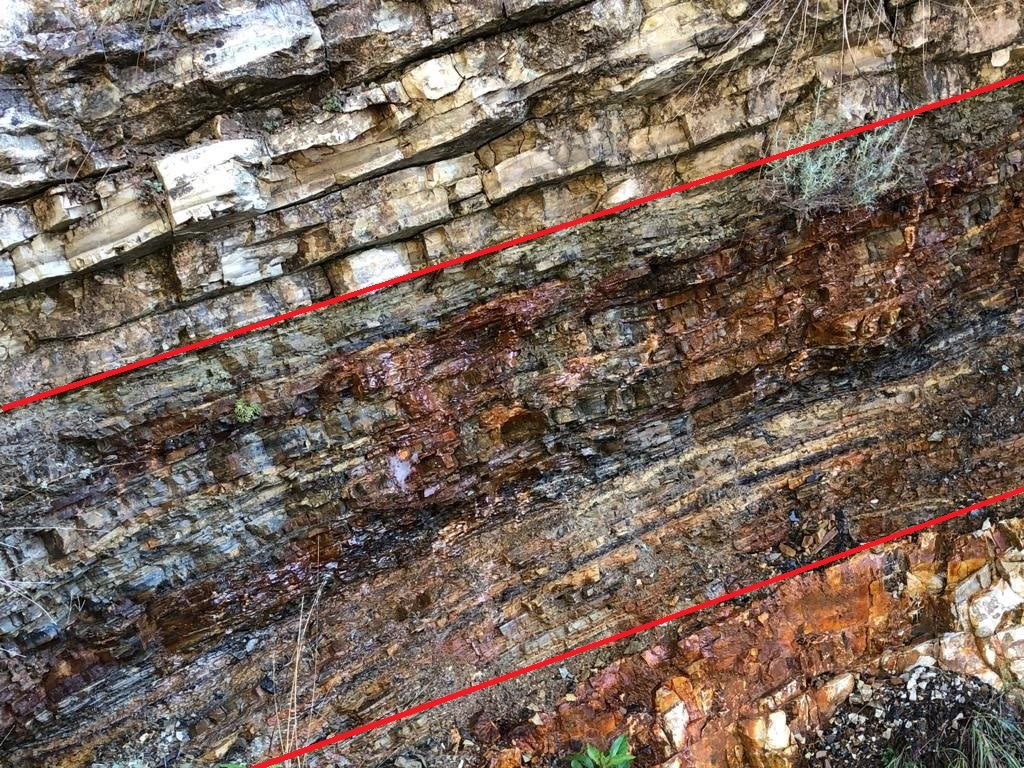
\includegraphics[width=0.66\linewidth]{images/book4/b2-19-bonarelli-level.jpg}
\par\smallskip{\small Het Bonarelli-niveau, de donkere schalie van OAE~2, tussen bleke kalkstenen; de
rode lijnen, door de fotograaf getekend, geven de basis en de top aan. (Picenus, CC~BY-SA~4.0, via
Wikimedia Commons.)}
\end{omfigure}
% ledger: rigo24:oaes

\begin{inthefield}[Een anoxische gebeurtenis opnemen]
Een geologe die een OAE bestudeert in een sectie van pelagische kalkstenen, neemt ze laag voor laag op: dikte,
kleur, laminatie, graafgangen of het ontbreken ervan, knollen van pyriet. Ze neemt monsters met kleine, regelmatige
tussenafstanden door het donkere interval en ver daarbuiten, voor het gehalte aan organische koolstof en voor de
koolstofisotopen van het organische materiaal en van het carbonaat; de verschuiving van de isotopen, meer dan
de kleur van het gesteente, correleert de gebeurtenis van het ene bekken naar het andere. Omdat de donkerste
schalie in verschillende bekkens op verschillende niveaus kan verschijnen, wordt de isotopencurve, niet de zwarte
schalie, als tijdlijn genomen.
\end{inthefield}
% ledger: rigo24:oaes, wt24:oae2

\subsection*{Chicxulub}

Het einde van het Krijt had een oorzaak van buitenaf. Boek~3 vertelde hoe het iridium van de
grensklei naar een inslag leidde, en hoe argondatering de grens aan de Chicxulub-krater koppelde.
De structuur is ongeveer \qty{200}{km} breed en \qty{66}{Ma} oud; haar
hete gesteenten voedden circulerend water gedurende minstens acht miljoen jaar daarna. Modellen van haar ondergrondse
asymmetrie wijzen op een inslaglichaam dat uit het noordoosten kwam onder 45 tot \ang{60} met de horizontaal,
met niet minder dan de ontsnappingssnelheid van de Aarde, \qty{11.2}{km.s^{-1}}, en waarschijnlijker ongeveer
\qty{20}{km.s^{-1}}. De Deccan-trappen waren tegelijk in uitbarsting, vóór en na de
inslag; een overzicht van het bewijs in 2010 concludeerde dat de inslag het uitsterven in gang zette.
% ledger: pickersgill26:chicxulub, collins20:impact, renne:kpg, alvarez:iridium, schulte:kpg, cr03:deccan

\begin{dated}{2026}
De ouderdommen in dit hoofdstuk zijn die van de Internationale Chronostratigrafische Kaart in haar versie van juni
2026, zoals in deze hele reeks gebruikt; de zeeniveaureeksen staan op de tijdschaal van 2012
van hun bestanden, en de uitstervingsouderdommen zijn die van Kaiho (2022). De kaart wordt herzien naarmate nieuwe
dateringen binnenkomen: raadpleeg de huidige versie voordat een grensouderdom wordt geciteerd.
\end{dated}
% ledger: ics:base.Phanerozoic, data:b4-sealevel, kaiho22:table

\section*{Oefeningen}\label{sec:b2:phanerozoic-earth:exercises}

Gegevens voor de oefeningen, tenzij anders vermeld: \qty{111.2}{km} per breedtegraad; diepte
van de oceaanbodem $d(t) = 2500 + 350\sqrt t$ (\unit{m}, $t$ in \unit{Myr}); oceaanoppervlakte
\qty{362}{\mega km^2}; oppervlakte van de oceaanbodem \qty{293}{\mega km^2}; dichtheid van de mantel
\qty{3300}{kg.m^{-3}}; zeewater \qty{1025}{kg.m^{-3}}; massa van de atmosfeer
\qty{5.1e18}{kg}, molaire massa's van lucht en van koolstofdioxide \qty{28.97}{g.mol^{-1}} en
\qty{44.01}{g.mol^{-1}}.
% ledger: earth:Rmean, ps77:depth-age, charette:ocean-volume, data:b4-ridge, katz03:thermo, noaa:seawater-1025, earth:Matm, earth:Mmol, ciaaw:abridged-2024

\begin{exercise}[$\star$]\label{exo:b2:phanerozoic-earth:1}
In het model van de kaarten lag Kaapstad \qty{300}{Ma} geleden op \ang{61.9}~ZB en New York op
\ang{3.6}~ZB; vandaag liggen ze op \ang{33.9}~ZB en \ang{40.7}~NB. (a) Welke van de vier steden lag
\qty{300}{Ma} geleden binnen \ang{30} van de evenaar (Parijs op \ang{5.1}~NB, Sydney op
\ang{59.5}~ZB)? (b) Hoe ver naar het noorden, in kilometer, zijn Kaapstad en New York elk sindsdien verschoven?
(c) Met welke gemiddelde snelheden, in centimeter per jaar?
\end{exercise}
% ledger: data:b4-palaeopos, geonames4:cities

\begin{exercise}[$\star$]\label{exo:b2:phanerozoic-earth:2}
De grote vijf vielen op 444, 372, 251.9, 201.4 en \qty{66}{Ma}. (a) Bepaal de intervallen tussen
opeenvolgende crises en hun gemiddelde. (b) Welke van de vijf vallen, met de gemiddelde ouderdommen van de grote stollingsprovincies ---
Emeishan 259, Siberië 250, CAMP 201, Karoo--Ferrar 183, Deccan \qty{65.5}{Ma} --- binnen \qty{2}{Myr} van een provincie?
(c) Maakt een gemiddeld interval de crises periodiek?
\end{exercise}
% ledger: kaiho22:table, cr03:table

\begin{exercise}[$\star$]\label{exo:b2:phanerozoic-earth:3}
Het krijt van Monument Rocks werd afgezet met ongeveer \qty{0.036}{mm} per jaar. (a) Hoe lang duurde
\qty{91}{m} ervan? (b) Hoeveel keer sneller stijgt de zee vandaag, met \qty{3.7}{mm} per
jaar? (c) Waarom kan een zeebodem zo'n trage regen van sediment verzamelen zonder door modder te worden begraven?
\end{exercise}
% ledger: kgs:monument-rocks, ipcc:sea-level-obs

\begin{exercise}[$\star$]\label{exo:b2:phanerozoic-earth:4}
In een klif, van onder naar boven: rivierzandsteen met wortels, strandzand met schelpen, grijze offshore-modder,
krijt; daarna wordt het krijt opnieuw bedekt door strandzand. (a) Waar legt de sectie een
\omterm{def:b2:phanerozoic-earth:transgression}{mariene transgressie} vast, en waar een regressie? (b) Bewijst de transgressie dat het wereldwijde
zeeniveau steeg? (c) Wat zou haar overtuigender maken?
\end{exercise}

\begin{exercise}[$\star\star$]\label{exo:b2:phanerozoic-earth:5}
Op de langetermijncurve van Haq en anderen stond het zeeniveau \qty{233}{m} boven het huidige op
\qty{97}{Ma}. (a) Met welke gemiddelde snelheid is het sindsdien gedaald, in meter per miljoen jaar en in
micrometer per jaar? (b) Vergelijk met de huidige stijging van \qty{3.7}{mm} per jaar. (c) De gebackstripte
curve van New Jersey geeft op hetzelfde tijdstip ongeveer \qty{70}{m}. Welke curve verdient voor de
amplitude het meeste vertrouwen, en waarom?
\end{exercise}
% ledger: data:b4-sealevel, ipcc:sea-level-obs, miller05:abstract, miller20:epr

\begin{exercise}[$\star\star$]\label{exo:b2:phanerozoic-earth:6}
Eén enkele puls van de CAMP, ongeveer \qty{e5}{km^3} basalt met dichtheid \qty{2900}{kg.m^{-3}},
barstte uit in ongeveer 500 jaar. (a) Hoeveel gaf ze af met \qty{0.75}{\percent} koolstofdioxide in massa,
in kilogram en in mol? (b) Welke massa koolstofdioxide bevatte de lucht bij
de \qty{278}{ppm} van 1750? (c) Vergelijk. (d) Hoeveel zulke atmosferen zou de hele provincie,
\qty{e5}{Gt}, hebben geleverd?
\end{exercise}
% ledger: capriolo20:camp-co2, ipcc:erf-2xco2, earth:Matm, earth:Mmol, ciaaw:abridged-2024

\begin{exercise}[$\star\star$]\label{exo:b2:phanerozoic-earth:7}
Neem het inslaglichaam van Chicxulub als een bol met een diameter van \qty{10}{km} en een dichtheid van
\qty{2630}{kg.m^{-3}}. (a) Bepaal zijn massa. (b) Bepaal zijn kinetische energie bij de kleinst mogelijke
snelheid, \qty{11.2}{km.s^{-1}}, en bij \qty{20}{km.s^{-1}}. (c) De Aarde verliest \qty{47}{TW}
inwendige warmte door haar oppervlak. Met hoeveel jaar van dat verlies komt elke energie overeen?
\end{exercise}
% ledger: alvarez:iridium, collins20:impact, b2dd10:half-space

\begin{exercise}[$\star\star$]\label{exo:b2:phanerozoic-earth:8}
(a) Noem de kenmerken waarmee een zwarte schalie een \omterm{def:b2:phanerozoic-earth:oae}{oceanische anoxische gebeurtenis} vastlegt. (b) Koppel elke
gebeurtenis aan een provincie van bijna dezelfde ouderdom: vroeg Toarcien, \qty{183}{Ma}; OAE~1a,
\qty{120}{Ma}; gegeven Karoo--Ferrar op \qty{183}{Ma} en Ontong Java op \qty{122}{Ma}. (c) Waarom is een
samenvallen van ouderdommen niet genoeg om te bewijzen dat een provincie een gebeurtenis veroorzaakte?
\end{exercise}
% ledger: rigo24:oaes, cr03:table

\begin{exercise}[$\star\star$]\label{exo:b2:phanerozoic-earth:9}
In het model lag Parijs \qty{500}{Ma} geleden op \ang{60.9}~ZB en \qty{300}{Ma} geleden op \ang{5.1}~NB.
(a) Bepaal zijn noordwaartse verplaatsing in graden en in kilometer, en de gemiddelde snelheid in
centimeter per jaar. (b) Vergelijk met de snelheid sinds \qty{300}{Ma}
(\cref{ex:b2:phanerozoic-earth:paris}). (c) Waarom is de snelheid een minimum?
\end{exercise}
% ledger: data:b4-palaeopos

\begin{exercise}[$\star\star\star$]\label{exo:b2:phanerozoic-earth:10}
Veronderstel in plaats daarvan dat de oppervlakte van de bodem lineair afneemt met de ouderdom, van een maximum op ouderdom 0 tot nul
op ouderdom $T$. (a) Toon aan dat de gemiddelde ouderdom $T/3$ is en dat het gemiddelde van $\sqrt t$ gelijk is aan
$\tfrac{8}{15}\sqrt T$. (b) Bepaal met een gemiddelde ouderdom van \qty{64.2}{Myr} $T$ en de gemiddelde diepte. (c)
Bepaal de daling van de gemiddelde diepte wanneer de spreidingssnelheid verdubbelt, en vergelijk met de
\qty{774}{m} van het gelijkmatige model. (d) Toon aan dat in beide modellen de daling dicht bij $0.93\,c\sqrt{\bar
t}\,(1 - f^{-1/2})$ ligt, met $\bar t$ de gemiddelde ouderdom.
\end{exercise}

\begin{exercise}[$\star\star\star$]\label{exo:b2:phanerozoic-earth:11}
(a) Toon uitgaande van \cref{prop:b2:phanerozoic-earth:ridge} aan dat $\Delta s(f) = \Delta s(2)\,(1 -
f^{-1/2})/(1 - 2^{-1/2})$. (b) Bepaal met $\Delta s(2) = \qty{432}{m}$ het bereik van $f$ dat
de krijtpiek geeft, 50 tot \qty{150}{m}. (c) Wat zou een spreidingssnelheid doen die vertraagd is tot 0.8 van
de huidige? (d) Waarom is een langetermijnzeeniveau dat door ruggen wordt bepaald een traag signaal, wat de verandering van
snelheid ook is?
\end{exercise}
% ledger: data:b4-ridge, miller05:abstract

\begin{exercise}[$\star\star\star$]\label{exo:b2:phanerozoic-earth:12}
Veronderstel dat soorten met een constante snelheid uitsterven, zodat de fractie van een cohort die een tijd
$t$ overleeft $2^{-t/m}$ is, met een mediane levensduur van een soort $m = \qty{2}{Myr}$. (a) Welke fractie van een
cohort is verdwenen na \qty{7.4}{Myr}, de gemiddelde etagelengte van de analyse van 1982? (b) Hoe lang
zou achtergronduitsterving nodig hebben om \qty{81}{\percent} van de soorten te verwijderen? (c) De crisis aan het einde van het Perm
duurde ongeveer \qty{60}{kyr}. Hoeveel sneller was ze? (d) Waarom vervaagt een grove
tijdresolutie het verschil tussen een massa-uitsterving en een achtergronduitsterving?
\end{exercise}
% ledger: marshall23:resolution, stanley16:permian, burgess:end-permian

\begin{problem}[{Weekendprobleem --- Toen de ruggen snel waren}]\label{pb:b2:phanerozoic-earth:1}
Dit probleem vraagt hoeveel de zee zou stijgen, en hoeveel land ze zou laten verdrinken, als de
ruggen twee keer zo snel uiteenspreidden. Gebruik de gegevens van de oefeningen; de gemiddelde ouderdom van de oceaanbodem is
\qty{64.2}{Myr}, de ruggen zijn in totaal \qty{65000}{km} lang, de huidige oceaan bevat
\qty{1.33e9}{km^3}, en het land beslaat \qty{148}{\mega km^2}. De tabel geeft het percentage van het
huidige land dat minder dan $h$ boven zeeniveau ligt, uit het ETOPO1-raster van één graad.
\begin{center}
\small
\begin{tabular}{lcccccc}
\hline
$h$ (\unit{m}) & 0 & 100 & 200 & 300 & 400 & 500 \\
land onder $h$ (\unit{\percent}) & 0 & 14.9 & 28.2 & 38.7 & 48.1 & 55.8 \\
\hline
\end{tabular}
\end{center}
Neem aan, zoals in \cref{prop:b2:phanerozoic-earth:ridge}, dat elke ouderdom van de bodem tussen 0 en de
ouderdom $\tau$ waarop hij wordt gesubduceerd, dezelfde oppervlakte beslaat.

\noindent\textbf{Deel I --- De oceaanbodem vandaag.}
\begin{enumerate}
  \item Bepaal de diepte van de bodem op de ouderdommen 0, 25, 64.2 en \qty{100}{Myr}.
  \item Bepaal $\tau$ uit de gemiddelde ouderdom, en de diepte van de oudste bodem.
  \item Bepaal de gemiddelde volle spreidingssnelheid $u = A_{\text{f}}/(L\tau)$, in kilometer per miljoen
        jaar en in millimeter per jaar. Is het een trage, gemiddelde of snelle snelheid?
  \item Toon aan dat de gemiddelde diepte van de bodem $2500 + \tfrac23 \times 350\sqrt\tau$ is, en
        bereken ze.
  \item De gemeten gemiddelde diepte van de gedateerde bodem is \qty{4265}{m}. Geef twee redenen waarom het
        model dieper is.
  \item Welk volume water zou in het model boven de bodem liggen? Vergelijk met het volume van
        de hele oceaan.
\end{enumerate}

\noindent\textbf{Deel II --- Een rug in doorsnede.}
\begin{enumerate}[resume]
  \item Bepaal de halve spreidingssnelheid $v$, tot op \qty{0.1}{km.Myr^{-1}}, en de breedte
        van de bodem aan elke kant van de rug.
  \item Hoe diep ligt de bodem op \qty{1000}{km} van de as?
  \item Toon aan dat de doorsnede van de rug boven de diepte van de oudste bodem, met
        beide flanken meegerekend, de oppervlakte $\tfrac23 v c\,\tau^{3/2}$ heeft, en bereken ze in
        vierkante kilometer.
  \item Bepaal het volume van het hele ruggenstelsel boven die diepte.
  \item Welke fractie van het volume van de oceaan is dat?
  \item Waarom staat een rug die sneller uiteenspreidt gemiddeld hoger?
\end{enumerate}

\noindent\textbf{Deel III --- Twee keer zo snel.}
\begin{enumerate}[resume]
  \item De spreidingssnelheid verdubbelt bij dezelfde bodemoppervlakte en ruglengte. Bepaal de nieuwe $\tau$
        en de nieuwe gemiddelde diepte.
  \item Hoeveel daalt de gemiddelde diepte?
  \item Welk volume water duwt de bodem uit de bekkens?
  \item Hoeveel zou het de zee doen stijgen als het over de huidige oceaan werd verdeeld?
  \item Neem het wegzakken van de bodem onder het extra water mee om de stijging $\Delta s$ te vinden.
  \item De krijtpiek op lange termijn bedroeg ongeveer \qty{100}{m}. Welke toename van de spreidingssnelheid
        zou dat geven?
\end{enumerate}

\noindent\textbf{Deel IV --- De zee over het land.}
\begin{enumerate}[resume]
  \item Welke landoppervlakte zou een stijging van \qty{100}{m} overstromen?
  \item Welke oppervlakte zou een stijging van \qty{432}{m} overstromen, door interpolatie in de tabel?
  \item Waarom moet de zee minder dan \qty{432}{m} stijgen zodra ze zich over het land uitspreidt?
  \item Bepaal het volume dat nodig is om de zee in stappen van \qty{100}{m} tot \qty{400}{m} te verhogen,
        door de overstroomde oppervlakte over elke stap te middelen (\cref{prop:b2:phanerozoic-earth:flooding}).
        Het te plaatsen volume is $\qty{0.432}{km} \times \qty{362}{\mega km^2}$. Waar stopt
        de zee?
  \item Welk percentage van het huidige land bedekt ze dan?
  \item Samengevat: hoeveel zou een verdubbeling van de spreidingssnelheid de zee in dit model doen stijgen?
\end{enumerate}
\end{problem}
% ledger: ps77:depth-age, seton:mean-age, seton:rate-classes, noaa:ridge, charette:ocean-volume, data:b4-ridge, data:b4-floor-depth, katz03:thermo, noaa:seawater-1025, data:b4-hyps, miller05:abstract
